
Consider we want the following function to be a coroutine:

\begin{cpp}
void coro(int max)
{
	std::cout << "CORO " << max << " start\n";
	
	for (int val = 1; val <= max; ++val) {
		std::cout << "CORO " << val << '/' << max << '\n';
	}
	
	std::cout << "CORO " << max << " end\n";
}
\end{cpp}

This function has a parameter for the maximum value, which we first print. Then, it loops from 1 to this maximum value and prints each value. Finally, we have a print statement at the end.

When the function is called with coro(3), it has the following output:

\begin{shell}
CORO 3 start
CORO 1/3
CORO 2/3
CORO 3/3
CORO 3 end
\end{shell}

However, we want to program this as a coroutine that is suspended each time the print statement inside the loop is performed. Therefore, the function is interrupted and the user of the coroutine can trigger the next output with a resumption.

\mySubsubsection{14.2.1}{Defining the Coroutine}

Here is the complete code for the definition of the coroutine:

\filename{lib/atomicwait.cpp}

\begin{cpp}
#include <iostream>
#include "corotask.hpp" // for CoroTask

CoroTask coro(int max)
{
	std::cout << "             CORO " << max << " start\n";
	
	for (int val = 1; val <= max; ++val) {
		// print next value:
		std::cout << "          CORO " << val << '/' << max << '\n';
		
		co_await std::suspend_always{}; // SUSPEND
	}
	
	std::cout << " CORO " << max << " end\n";
}
\end{cpp}

We still have a kind of a function that loops over the values up to the parameter max. However, two things differ from ordinary functions:

\begin{itemize}
\item 
Inside the loop after the print statement, there is a co\_await expression, which suspends the coroutine and blocks it until it is resumed. This is called a suspend point.

The exact behavior of the suspend call is defined by the expression immediately after co\_await. It enables programmers to control the exact behavior of the suspension.

For the moment, we will use a default-constructed object of type std::suspend\_always, which accepts the suspension and gives control back to the caller. However, you can reject the suspension or resume another coroutine instead by passing special operands to co\_await.

\item 
Although the coroutine has no return statement, it has a return type, CoroTask. This type serves as the coroutine interface for the caller of the coroutine. Note that we cannot declare the return type as auto.

The return type is necessary because the caller needs an interface to be able to deal with the coroutine (such as resuming it). In C++20, coroutine interface types have to be provided by the programmer (or a third party library). We will see later how it is implemented. The plan is that upcoming C++ standards will provide some standard coroutine interface types in their library.
\end{itemize}

\mySubsubsection{14.2.2}{Using the Coroutine}

We can use the coroutine as follows:

\filename{coro/coro.cpp}

\begin{cpp}
#include <iostream>
#include "coro.hpp"

int main()
{
	// start coroutine:
	auto coroTask = coro(3); // initialize coroutine
	std::cout << "coro() started\n";
	
	// loop to resume the coroutine until it is done:
	while (coroTask.resume()) { // RESUME
		std::cout << "coro() suspended\n";
	}
	
	std::cout << "coro() done\n";
}
\end{cpp}

After initializing the coroutine, which yields the coroutine interface coroTask, we start a loop that again and again resumes the coroutine after it has been suspended:

\begin{cpp}
auto coroTask = coro(3); // initialize coroutine

while (coroTask.resume()) { // RESUME
	...
}
\end{cpp}

By calling coro(3), we call the coroutine like a function. However, in contrast to function calls, we do not wait for the coroutine to end. Instead, the call returns the coroutine interface to deal with the coroutine after the coroutine is initialized (there is an implicit suspend point at the beginning).

We use auto here for the coroutine interface type; however, we could also use its type, which is the return type of the coroutine:

\begin{cpp}
CoroTask coroTask = coro(3); // initialize coroutine
\end{cpp}

The API provided by the class CoroTask provides a member function resume(), which resumes the coroutine. Each call of resume() allows the coroutine to continue to run until the next suspension or until the end of the coroutine. Note that a suspension does not leave any scope in the coroutine. On resumption, we continue the coroutine in the state of its suspension.

The effect is that within the loop in main(), we call the next bunch of statements in the coroutine until we reach a suspend point or the end. That is, we call the following:

\begin{itemize}
\item 
First, the initial output, the initialization of val, and the first output inside the loop:

\begin{cpp}
std::cout << "                 CORO " << max << " start\n";
for (int val = 1; val <= max; ... ) {
	std::cout << "               CORO " << val << '/' << max << '\n';
	...
}
\end{cpp}

\item 
Then twice, the next iteration in the loop:

\begin{cpp}
	for (...; val <= max; ++val) {
		std::cout << "               CORO " << val << '/' << max << '\n';
		...
	}
\end{cpp}

\item 
Finally, after the last iteration in the loop, the coroutine performs the final print statement:

\begin{cpp}
for ( ... ; val <= max; ++val) {
	...
}

std::cout << " CORO " << max << " end\n";
\end{cpp}
\end{itemize}

The output of the program is as follows:

\begin{shell}
coro() started
         CORO 3 start
         CORO 1/3
coro() suspended
         CORO 2/3
coro() suspended
         CORO 3/3
coro() suspended
         CORO 3 end
coro() done
\end{shell}


\begin{center}
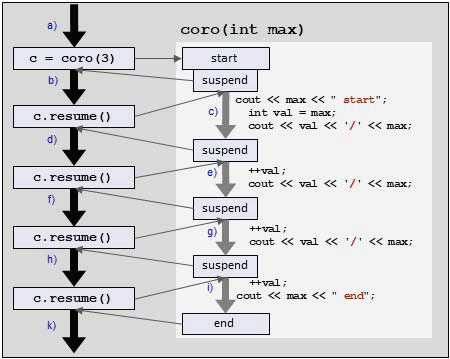
\includegraphics[width=0.6\textwidth]{content/chapter14/images/2.png}\\
Figure 14.2. Coroutine example
\end{center}

In combination with the interface type CoroTask, which we will see in a moment, we get the following control flow (see Figure 14.2):

\begin{enumerate}[label=\alph*)]
\item 
First, we call the coroutine so that it starts. The coroutine is immediately suspended and the call returns the interface object to deal with the coroutine.

\item 
We can then use the interface object to resume the coroutine so that it starts performing its statements.

\item 
Inside the coroutine we process the starting statements up to the first suspend point: the first print statement, the initialization of the local counter val in the head of the loop, and (after checking that val is less than or equal to max) the print statement inside the loop. At the end of this part, the coroutine is suspended.

\item 
The suspension transfers control back to the main function, which then continues until it resumes the coroutine again.

\item 
The coroutine continues performing the next statements until we reach the suspend point again, incrementing val and (after checking that val is still less than or equal to max) executing the print statement inside the loop. At the end of this part, the coroutine is suspended again.

Note that we continue here with the value that val had when the coroutine was suspended before.

\item 
This again transfers control back to the main function, which then continues until it resumes the coroutine once more.

\item 
The coroutine continues the loop as long as the incremented val is less than or equal to max.

\item 
The main function resumes the coroutine as long as the coroutine was suspended with co\_await.

\item 
Finally, the coroutine leaves the loop after val was incremented, which calls the final print statement with the value of max.

\item 
The end of the coroutine transfers control back to the main function for the last time. The main function then ends its loop and continues until its end.
\end{enumerate}

The exact behavior of the initialization and the interface of the coroutine depends on the interface type CoroTask. It might just start the coroutine or provide a context with some initializations, such as opening a file or starting a thread. It also defines whether the coroutine starts immediately or starts lazily (is immediately suspended). With the current implementation of CoroTask it starts lazily, which means that the initial call of the coroutine does not perform any statements of coro() yet.

Note that there is no asynchronous communication or control flow. It is more that coroTask.resume() is like a function call for the next portion of coro().

The loop ends when we have reached the end of the coroutine. For this purpose, resume() is implemented such that it returns whether the coroutine is not done (yet). Thus, while resume() returns true, we continue the loop (after printing that it was suspended).

\mySamllsection{Using Coroutines Multiple Times}

As written, a coroutine is kind of a quasi-parallel function, executed sequentially by switching the control flow back and forth. Its state is stored in some heap memory controlled by the coroutine handle, which is usually held by the coroutine interface. By having multiple coroutine interface objects, we can deal with the state of multiple active coroutines, which might be running or suspended independently of each other.

Assume that we start two coroutines with different values for max:

\filename{coro/coro2.cpp}

\begin{cpp}
#include <iostream>
#include "coro.hpp"

int main()
{
	// start two coroutines:
	auto coroTask1 = coro(3); // initialize 1st coroutine
	auto coroTask2 = coro(5); // initialize 2nd coroutine
	std::cout << "coro(3) and coro(5) started\n";
	
	coroTask2.resume(); // RESUME 2nd coroutine once
	
	// loop to resume the 1st coroutine until it is done:
	while (coroTask1.resume()) { // RESUME 1st coroutine
		std::cout << "coro() suspended\n";
	}
	
	std::cout << "coro() done\n";
	
	coroTask2.resume(); // RESUME 2nd coroutine again
}
\end{cpp}

We get two different interface objects, coroTask1 and coroTask2, for the initialized coroutines. By resuming sometimes the first and sometimes the second coroutine, our control flow jumps between the main function and these two coroutines.

In our case, we resume the second coroutine (having 5 as max) once, then loop over resuming the first coroutine, and finally resume the second coroutine once again. As a result, the program has the following output:

\begin{shell}
coro(3) and coro(5) started
         CORO 5 start
         CORO 1/5
         CORO 3 start
         CORO 1/3
coro() suspended
         CORO 2/3
coro() suspended
         CORO 3/3
coro() suspended
         CORO 3 end
coro() done
         CORO 2/5
\end{shell}

You can even pass the coroutine interface objects to different functions or threads to resume them there. They will always continue with their current state.

\mySubsubsection{14.2.3}{Lifetime Issues with Call-by-Reference}

A coroutine usually lives longer than the statement it was initially called from. That has an important consequence: you can run into fatal runtime problems if you pass temporary objects by reference.

Consider the following slightly modified coroutine. All we do now is take the max value by reference:

\filename{coro/cororef.hpp}

\begin{cpp}
#include <iostream>
#include <coroutine> // for std::suspend_always{}
#include "corotask.hpp" // for CoroTask

CoroTask coro(const int& max)
{
	std::cout << "   CORO " << max << " start\n"; // OOPS: value of max still valid?
	
	for (int val = 1; val <= max; ++val) { // OOPS: value of max still valid?
		std::cout << " CORO " << val << '/' << max << '\n';
		co_await std::suspend_always{}; // SUSPEND
	}
	
	std::cout << " CORO " << max << " end\n"; // OOPS: value of max still valid?
}
\end{cpp}

The problem is that passing a temporary object, which might even be a literal, creates undefined behavior. You might or might not see it depending on the platform, compiler settings, and the rest of the code. Consider, for example, calling the coroutine as follows:

\filename{coro/cororef.hpp}

\begin{cpp}
#include <iostream>
#include "cororef.hpp"

int main()
{
	auto coroTask = coro(3); // OOPS: creates reference to temporary/literal
	std::cout << "coro(3) started\n";
	coro(375); // another temporary coroutine
	std::cout << "coro(375) started\n";
	// loop to resume the coroutine until it is done:
	
	while (coroTask.resume()) { // ERROR: undefined behavior
		std::cout << "coro() suspended\n";
	}
	std::cout << "coro() done\n";
}
\end{cpp}

On some platforms this code works fine. However, on one platform where I tested this code, I got the following output:

\begin{shell}
coro(3) started
coro(375) started
  CORO -2147168984 start
  CORO -2147168984 end
coro() done
\end{shell}

After the statement that initializes the coroutine, the location the max reference refers to for the passed argument 3 is no longer available. Therefore, when resuming the coroutine for the first time, the output and initialization of val are using a reference to a destroyed object.

In general: \textbf{do not use references to declare coroutine parameters.}

If copying the parameter becomes too expensive, you can “pass by reference” by using reference wrappers created with std::ref() or std::cref(). For containers, you can use std::views::all() instead, which passes the container as a view, so that all standard range functions can still be used without converting the parameter back. For example:

\begin{cpp}
CoroTask printElems(auto coll)
{
	for (const auto& elem : coll) {
		std::cout << elem << '\n';
		co_await std::suspend_always{}; // SUSPEND
	}
}
std::vector<std::string> coll;
...
// start coroutine that prints the elements:
// - use view created with std::views::all() to avoid copying the container
auto coPrintElems = printElems(std::views::all(coll));

while (coPrintElems.resume()) { // RESUME
...
}
\end{cpp}

\mySubsubsection{14.2.4}{Coroutines Calling Coroutines}

Coroutines can call other coroutines (even indirectly) and both the calling and the called coroutines might have suspend points. Let us look at what that means.

Consider a coroutine with one suspend point so that it runs in two parts:

\begin{cpp}
CoroTask coro()
{
	std::cout << " coro(): PART1\n";
	co_await std::suspend_always{}; // SUSPEND
	std::cout << " coro(): PART2\n";
}
\end{cpp}

When we use this coroutine as follows:

\begin{cpp}
auto coroTask = coro(); // initialize coroutine
std::cout << "MAIN: coro() initialized\n";

while (coroTask.resume()) { // RESUME
	std::cout << "MAIN: coro() suspended\n";
}

std::cout << "MAIN: coro() done\n";
\end{cpp}

We get the following output:

\begin{shell}
MAIN: coro() initialized
    coro(): PART1
MAIN: coro() suspended
    coro(): PART2
MAIN: coro() done
\end{shell}

Now let us call coro() indirectly via another coroutine. For that, main() calls callCoro() instead of coro():

\begin{cpp}
auto coroTask = callCoro(); // initialize coroutine
std::cout << "MAIN: callCoro() initialized\n";

while (coroTask.resume()) { // RESUME
	std::cout << "MAIN: callCoro() suspended\n";
}

std::cout << "MAIN: callCoro() done\n";
\end{cpp}

The interesting part is how to implement callCoro().

\mySamllsection{No Inner resume()}

We might try to implement callCoro() by just calling coro():

\begin{cpp}
CoroTask callCoro()
{
	std::cout << " callCoro(): CALL coro()\n";
	coro(); // CALL sub-coroutine
	std::cout << " callCoro(): coro() done\n";
	co_await std::suspend_always{}; // SUSPEND
	std::cout << " callCoro(): END\n";
}
\end{cpp}

This compiles. However, it does not work as expected, as the output of the program demonstrates:

\begin{shell}
MAIN: callCoro() initialized
  callCoro(): CALL coro()
  callCoro(): coro() done
MAIN: callCoro() suspended
  callCoro(): END
MAIN: callCoro() done
\end{shell}

The print statements in the body of coro() are never called.

The reason is that

\begin{cpp}
coro();
\end{cpp}

only initializes the coroutine and immediately suspends it. coro() is never resumed. It cannot be resumed because the coroutine interface returned is not even used. A resume() of the outer coroutine does not automatically resume any inner coroutine.

To get at least a compiler warning when using coroutines like functions, class CoroTask will be declared with [[nodiscard]].

\mySamllsection{Using an Inner resume()}

We have to deal with the inner coroutine the same way we deal with the outer coroutine: resume() it in a loop:

\begin{cpp}
CoroTask callCoro()
{
	std::cout << " callCoro(): CALL coro()\n";
	auto sub = coro(); // init sub-coroutine
	while (sub.resume()) { // RESUME sub-coroutine
		std::cout << " callCoro(): coro() suspended\n";
	}
	std::cout << " callCoro(): coro() done\n";
	co_await std::suspend_always{}; // SUSPEND
	std::cout << " callCoro(): END\n";
}
\end{cpp}

With this implementation of callCoro(), we get the behavior and output we want:

\begin{shell}
MAIN: callCoro() initialized
  callCoro(): CALL coro()
    coro(): PART1
  callCoro(): coro() suspended
    coro(): PART2
  callCoro(): coro() done
MAIN: callCoro() suspended
  callCoro(): END
MAIN: callCoro() done
\end{shell}

See coro/corocoro.cpp for the complete example.

\mySamllsection{Using One Inner resume()}

It is worth noting what happens if we resume coro() inside callCoro() only once:

\begin{cpp}
CoroTask callCoro()
{
	std::cout << " callCoro(): CALL coro()\n";
	auto sub = coro(); // init sub-coroutine
	sub.resume(); // RESUME sub-coroutine
	std::cout << " callCoro(): call.resume() done\n";
	co_await std::suspend_always{}; // SUSPEND
	std::cout << " callCoro(): END\n";
}
\end{cpp}

The output becomes:

\begin{shell}
MAIN: callCoro() initialized
  callCoro(): CALL coro()
    coro(): PART1
  callCoro(): call.resume() done
MAIN: callCoro() suspended
  callCoro(): END
MAIN: callCoro() done
\end{shell}

After callCoro() initializes coro(), coro() is resumed only once, which means that only the first part of it is called. After that, the suspension of coro() transfers the control flow back to callCoro(), which then suspends itself, meaning that the control flow goes back to main(). When main() resumes callCoro(), the program finishes callCoro(). coro() is never finished at all.

\mySamllsection{Delegating resume()}

It is possible to implement CoroTask so that co\_await registers a sub-coroutine in a way that a suspension in the sub-coroutine is handled like a suspension in the calling coroutine. callCoro() would then look as follows:

\begin{cpp}
CoroTaskSub callCoro()
{
	std::cout << " callCoro(): CALL coro()\n";
	co_await coro(); // call sub-coroutine
	std::cout << " callCoro(): coro() done\n";
	co_await std::suspend_always{}; // SUSPEND
	std::cout << " callCoro(): END\n";
}
\end{cpp}

However, resume() then has to delegate a request for resumption to the sub-coroutine if there is one. For this purpose, the CoroTask interface has to become an awaitable. Later, after we have introduced awaitables, we will see such a coroutine interface that delegates resumptions to sub-coroutines.

\mySubsubsection{14.2.5}{Implementing the Coroutine Interface}

I have stated a couple of times that in our example, class CoroTask plays an important role for dealing with the coroutine. It is the interface that both the compiler and the caller of a coroutine usually deal with. The coroutine interface brings together a couple of requirements to let the compiler deal with coroutines and provides the API for the caller to create, resume, and destroy the coroutine. Let us elaborate on that in detail.

To deal with coroutines in C++ we need two things:

\begin{itemize}
\item 
A promise type 

This type is used to define certain customization points for dealing with a coroutine. Specific member functions define callbacks that are called in certain situations.

\item 
An internal coroutine handle of the type std::coroutine\_handle<>

This object is created when a coroutine is called (using one of the standard callbacks of the promise type above). It can be used to manage the state of the coroutine by providing a low-level interface to resume a coroutine as well as to deal with the end of the coroutine.
\end{itemize}

The usual purpose of the type dealing with the return type of a coroutine is to bring these requirements together:

\begin{itemize}
\item 
It has to define which promise type is used (it is usually defined as the type member promise\_type).

\item 
It has to define where the coroutine handle is stored (it is usually defined as a data member).

\item 
It has to provide the interface for the caller to deal with the coroutine (the member function resume() in this case).
\end{itemize}

\mySamllsection{The Coroutine Interface CoroTask}

The class CoroTask, which provides promise\_type, stores the coroutine handle, and defines the API for the caller of the coroutine, may be defined as follows:

\filename{coro/corotask.hpp}

\begin{cpp}
#include <coroutine>

// coroutine interface to deal with a simple task
// - providing resume() to resume the coroutine
class [[nodiscard]] CoroTask {
public:
	// initialize members for state and customization:
	struct promise_type; // definition later in corotaskpromise.hpp
	using CoroHdl = std::coroutine_handle<promise_type>;
	private:
	CoroHdl hdl; // native coroutine handle
	
public:
	// constructor and destructor:
	CoroTask(auto h)
	: hdl{h} { // store coroutine handle in interface
	}
	~CoroTask() {
		if (hdl) {
			hdl.destroy(); // destroy coroutine handle
		}
	}
	// don’t copy or move:
	CoroTask(const CoroTask&) = delete;
	CoroTask& operator=(const CoroTask&) = delete;
	
	// API to resume the coroutine
	// - returns whether there is still something to process
	bool resume() const {
		if (!hdl || hdl.done()) {
			return false; // nothing (more) to process
		}
		hdl.resume(); // RESUME (blocks until suspended again or the end)
		return !hdl.done();
	}
};

#include "corotaskpromise.hpp" // definition of promise_type
\end{cpp}

In the class CoroTask, we first define the basic types and member to deal with the native API of the coroutine. The key member the compiler looks for in a coroutine interface type is the type member promise\_type. With the promise type, we define the type of the coroutine handle and introduce a private member where this coroutine handle, specialized for the promise type, is stored:

\begin{cpp}
class [[nodiscard]] CoroTask {
public:
	// initialize members for state and customization:
	struct promise_type; // definition later in corotaskpromise.hpp
	using CoroHdl = std::coroutine_handle<promise_type>;
private:
	CoroHdl hdl; // native coroutine handle
	...
};
\end{cpp}

We introduce the promise\_type (which every coroutine type has to have) and declare the native coroutine handle hdl, which manages the state of the coroutine. As you can see, the type of the native coroutine handle, std::coroutine\_handle<>, is parameterized with the promise type. That way, any data stored in the promise is part of the handle and the functions in the promise are available via the handle.

The promise type has to be public to be visible from the outside. It is often also helpful to provide a public name of the type of the coroutine handle (CoroHdl in this case). To simplify things, we could even make the handle itself public. That way, we can use

\begin{cpp}
CoroTask::CoroHdl
\end{cpp}

instead of

\begin{cpp}
std::coroutine_handle<CoroTask::promise_type>
\end{cpp}

We could also define the promise type here directly inline. However, in this example, we defer the definition to the later included corotaskpromise.hpp.

The constructor and destructor of the coroutine interface type initialize the member for the coroutine handle and clean it up before the coroutine interface is destroyed:

\begin{cpp}
class CoroTask {
	...
	public:
	CoroTask(auto h)
	: hdl{h} { // store coroutine handle internally
	}
	~CoroTask() {
		if (hdl) {
			hdl.destroy(); // destroy coroutine handle (if there is one)
		}
	}
	...
};
\end{cpp}

By declaring the class with [[nodiscard]], we force compiler warnings when the coroutine is created but not used (which might especially happen by accidentally using a coroutine as an ordinary function).

For simplicity, we disable copying and moving. Providing copy or move semantics is possible but you have to be careful to deal with the resources correctly.

Finally, we define our only interface for the caller, resume():

\begin{cpp}
class CoroTask {
	...
	bool resume() const {
		if (!hdl || hdl.done()) {
			return false; // nothing (more) to process
		}
		hdl.resume(); // RESUME (blocks until suspended again or the end)
		return !hdl.done();
	}
};
\end{cpp}

The key API is resume(), which resumes the coroutine when it is suspended. It more or less propagates the request to resume to the native coroutine handle. It also returns whether it makes sense to resume the coroutine again.

First, the function checks whether we have a handle at all or whether the coroutine has already ended.

Even though in this implementation the coroutine interface always has a handle, this is a safety net which is necessary, for example, if the interface supports move semantics.

Calling resume() is only allowed when the coroutine is suspended and has not reached its end. Therefore, checking whether it is done() is necessary. The call itself resumes the suspended coroutine and blocks until it reaches the next suspend point or the end.

\begin{cpp}
hdl.resume(); // RESUME (blocks until suspended again or the end)
\end{cpp}

You can also use operator() for this:

\begin{cpp}
hdl(); // RESUME (blocks until suspended again or the end)
\end{cpp}

Because our resume() interface for the caller returns whether it makes sense to resume the coroutine again, we return whether the coroutine has reached its end:

\begin{cpp}
bool resume() const {
	...
	return !hdl.done();
}
\end{cpp}

The member function done() is provided by the native coroutine handle just for that purpose.

As you can see, the interface for the caller of the coroutine wraps the native coroutine handle and its API completely. In this API, we decide how the caller can deal with the coroutine. We could use different function names or even operators or split the calls for resumption and checking for the end. Later on you will see examples where we iterate over values the coroutine delivers with each suspension, we can even send values back to the coroutine, and we can provide an API to put the coroutine in a different context.

Finally, we include a header file with the definition of the promise type:

\begin{cpp}
#include "corotaskpromise.hpp" // definition of promise_type
\end{cpp}

This is usually done inside the declaration of the interface class or at least in the same header file. However, this way, we can split the details of this example over different files.

\mySamllsection{Implementing promise\_type}

The only missing piece is the definition of the promise type. Its purpose is to:

\begin{itemize}
\item 
Define how to create or get the return value of the coroutine (which usually includes creating the coroutine handle)

\item 
Decide whether the coroutine should suspend at its beginning or end

\item 
Deal with values exchanged between the caller of the coroutine and the coroutine

\item 
Deal with unhandled exceptions
\end{itemize}

Here is a typical basic implementation of the promise type for CoroTask and its coroutine handle type CoroHdl:

\filename{coro/corotaskpromise.hpp}

\begin{cpp}
struct CoroTask::promise_type {
	auto get_return_object() { // init and return the coroutine interface
		return CoroTask{CoroHdl::from_promise(*this)};
	}
	auto initial_suspend() { // initial suspend point
		return std::suspend_always{}; // - suspend immediately
	}
	void unhandled_exception() { // deal with exceptions
		std::terminate(); // - terminate the program
	}
	void return_void() { // deal with the end or co_return;
	}
	auto final_suspend() noexcept { // final suspend point
		return std::suspend_always{}; // - suspend immediately
	}
};
\end{cpp}
	
We (have to) define the following members (using the typical order in which they are used):

\begin{itemize}
\item 
get\_return\_object() is called to initialize the coroutine interface. It creates the object that is later returned to the caller of the coroutine. It is usually implemented as follows:
\begin{itemize}
\item 
First, it creates the native coroutine handle for the promise that we call this function for:

\begin{cpp}
coroHdl = CoroHdl::from_promise(*this)
\end{cpp}

The promise that we call this member function for is automatically created when we start the coroutine.

from\_promise() is a static member function that the class template std::coroutine\_handle<> provides for this purpose.

\item 
Then, we create the coroutine interface object, initializing it with the handle just created:

\begin{cpp}
coroIf = CoroTask{coroHdl}
\end{cpp}


\item 
Finally, we return the interface object:

\begin{cpp}
return coroIf
\end{cpp}

\end{itemize}

The implementation does this all in one statement:

\begin{cpp}
auto get_return_object() {
	return CoroTask{CoroHdl::from_promise(*this)};
}
\end{cpp}

We could also return the coroutine handle here without explicitly creating the coroutine interface from it:

\begin{cpp}
auto get_return_object() {
	return CoroHdl::from_promise(*this);
}
\end{cpp}

Internally, the returned coroutine handle is then automatically converted by using it to initialize the coroutine interface. However, this approach is not recommended, because it does not work if the constructor of CoroTask is explicit and because it is not clear when the interface is created.

\item 
initial\_suspend() allows additional initial preparations and defines whether the coroutine should start eagerly or lazily:

\begin{itemize}
\item 
Returning std::suspend\_never\{\} means starting eagerly. The coroutine starts immediately after its initialization with the first statements.

\item 
Returning std::suspend\_always\{\} means starting lazily. The coroutine is suspended immediately without executing any statement. It is processed with the resumption.
\end{itemize}

In our example, we request immediate suspension.

\item 
return\_void() defines the reaction when reaching the end (or a co\_return; statement). it this member function is declared, the coroutine should never return a value. If the coroutine yields or returns data, you have to use another member function instead.

\item 
unhandled\_exception() defines how to deal with exceptions not handled locally in the coroutine. Here, we specify that this results in an abnormal termination of the program. Other ways of dealing with exceptions are discussed later.

\item
final\_suspend() defines whether the coroutine should be finally suspended. Here, we specify that we want to do so, which is usually the right thing to do. Note that this member function has to guarantee not to throw exceptions. It should always return std::suspend\_always\{\}.
\end{itemize}

The purpose and use of these members of the promise type are discussed in detail later.

\mySubsubsection{14.2.6}{Bootstrapping Interface, Handle, and Promise}

Let us recapitulate what we need to deal with a coroutine:

\begin{itemize}
\item 
For each coroutine we have a promise, which is created automatically when a coroutine is called.

\item 
The coroutine state is stored in a coroutine handle. It has the type std::coroutine\_handle<PrmType>. That type provides the native API to resume a coroutine (and check whether it is at its end or destroy its memory).

\item 
The coroutine interface is the typical place to bring everything together. It holds and manages the native coroutine handle, it is returned by the call of the coroutine, and it provides member functions to deal with the coroutine.
\end{itemize}

There are various ways to declare the promise type and the coroutine handle (and the type of both). There is no obvious way to do it because the type of the coroutine handle needs the promise type and the definition of the promise type uses the coroutine handle.

In practice, the following options are usually used:

\begin{itemize}
\item 
Declare the promise type, declare the type of the coroutine handle, and define the promise type:

\begin{cpp}
class CoroTask {
public:
	struct promise_type; // promise type
	using CoroHdl = std::coroutine_handle<promise_type>;
private:
	CoroHdl hdl; // native coroutine handle
public:
	struct promise_type {
		auto get_return_object() {
			return CoroTask{CoroHdl::from_promise(*this)};
		}
		...
	};
	...
};
\end{cpp}

\item 
Define the promise type and declare the coroutine handle:

\begin{cpp}
class CoroTask {
public:
	struct promise_type { // promise type
		auto get_return_object() {
			return std::coroutine_handle<promise_type>::from_promise(*this);
		}
		...
	};
private:
	std::coroutine_handle<promise_type> hdl; // native coroutine handle
	public:
	...
};
\end{cpp}

\item 
Define the promise type outside as a generic helper type:

\begin{cpp}
template<typename CoroIf>
struct CoroPromise {
	auto get_return_object() {
		return std::coroutine_handle<CoroPromise<CoroIf>>::from_promise(*this);
	}
	...
};

class CoroTask {
	public:
	using promise_type = CoroPromise<CoroTask>;
	private:
	std::coroutine_handle<promise_type> hdl; // native coroutine handle
	public:
	...
};
\end{cpp}
\end{itemize}

Because the promise type is often interface-specific (having different/additional members), I usually use the following very condensed form:

\begin{cpp}
class CoroTask {
public:
	struct promise_type;
	using CoroHdl = std::coroutine_handle<promise_type>;
private:
	CoroHdl hdl; // native coroutine handle
public:
	struct promise_type {
		auto get_return_object() { return CoroHdl::from_promise(*this); }
		auto initial_suspend() { return std::suspend_always{}; }
		void return_void() { }
		void unhandled_exception() { std::terminate(); }
		auto final_suspend() noexcept { return std::suspend_always{}; }
		...
	};
	...
};
\end{cpp}

Note that everything described so far is kind of the typical way to deal with coroutines. There is more flexibility designed into the coroutine library. For example:

\begin{itemize}
\item 
You can store or manage coroutine interfaces in a container or scheduler.

\item 
You can even skip the coroutine interface completely. However, this is an option that is very rarely used.
\end{itemize}

\mySubsubsection{14.2.7}{Memory Management}

Coroutines have a state that is used in different contexts. For this purpose, a coroutine handle usually stores the state of a coroutine in heap memory. The heap memory allocation can be optimized away or pragmatically changed.

\mySamllsection{Calling destroy()}

To make coroutine handles cheap, there is no smart handling of this memory. Coroutine handles just point to the memory when initialized until destroy() is called. Therefore, you should usually call destroy() explicitly when the coroutine interface is destroyed:

\begin{cpp}
class CoroTask {
	...
	CoroHdl hdl; // native coroutine handle
	
	public:
	~CoroTask() {
		if (hdl) {
			hdl.destroy(); // destroy coroutine handle (if there is one)
		}
	}
	...
};
\end{cpp}

\mySamllsection{Copying and Moving Coroutines}

The cheap/naive implementation of coroutine handles also makes it necessary to deal with copying and moving. By default, copying the coroutine interface would copy the coroutine handle, which would have the effect that two coroutine interfaces/handles share the same coroutine. This, of course, introduces risks when one coroutine handle brings the coroutine into a state that the other handle is not aware of. Moving coroutine objects has the same effect, because by default, pointers are copied with a move.

To reduce the danger, you should be careful about providing copy or move semantics for coroutines. The easiest approach is to disable copying and moving:

\begin{cpp}
class CoroTask {
	...
	// don’t copy or move:
	CoroTask(const CoroTask&) = delete;
	CoroTask& operator=(const CoroTask&) = delete;
	...
};
\end{cpp}

However, this then means that you cannot move coroutines around (such as storing them in a container). Therefore, it might make sense to support move semantics. However, you should ensure that the movedfrom object no longer refers to the coroutine and that a coroutine that gets a new value destroys the data for the old one:

\begin{cpp}
class CoroTask {
	...
	// support move semantics:
	CoroTask(CoroTask&& c) noexcept
	: hdl{std::move(c.hdl)} {
		c.hdl = nullptr;
	}
	CoroTask& operator=(CoroTask&& c) noexcept {
		if (this != &c) { // if no self-assignment
			if (hdl) {
				hdl.destroy(); // - destroy old handle (if there is one)
			}
			hdl = std::move(c.hdl); // - move handle
			c.hdl = nullptr; // - moved-from object has no handle anymore
		}
		return *this;
	}
	...
};
\end{cpp}

Strictly speaking, you do not need std::move() for the handle here, but it does not hurt and reminds you that we delegate the move semantics to the member.











